
\noindent\textbf{9. (CRLS 22.3-7)} Mostre um contraexemplo para a conjectura que se existe um caminho de $u$ a $v$ em um grafo orientado $G$, e se $d[u] < d[v]$ numa DFS de $G$, então $v$ é descendente de $u$ na floresta DFS produzida.

Podemos observar a própria árvore à esquerda da figura 22.5 (c) do CLRS como um contraexemplo. Seja a DFS produzida a partir de $s$, se tomarmos os vértices $x$ e $w$, $d[x] < d[w]$, existe um caminho de $x$ a $w$, mas $w$ não é descendente de $x$.
\begin{center}
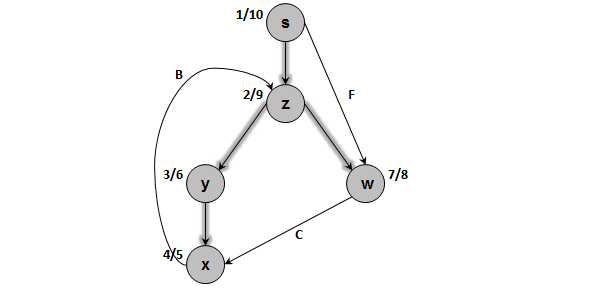
\includegraphics[width=0.8\textwidth]{q7-09.png}
\captionof{figure}{Contraexemplo utilizando parte do grafo da figura 22.5 (c) do CLRS.}
\label{fig:7.9-1}
\end{center}